\begin{figure}
	\centering
	\pgfplotsset{every axis legend/.append style={
		at={(1.05,0.5)},
		anchor=west}}
	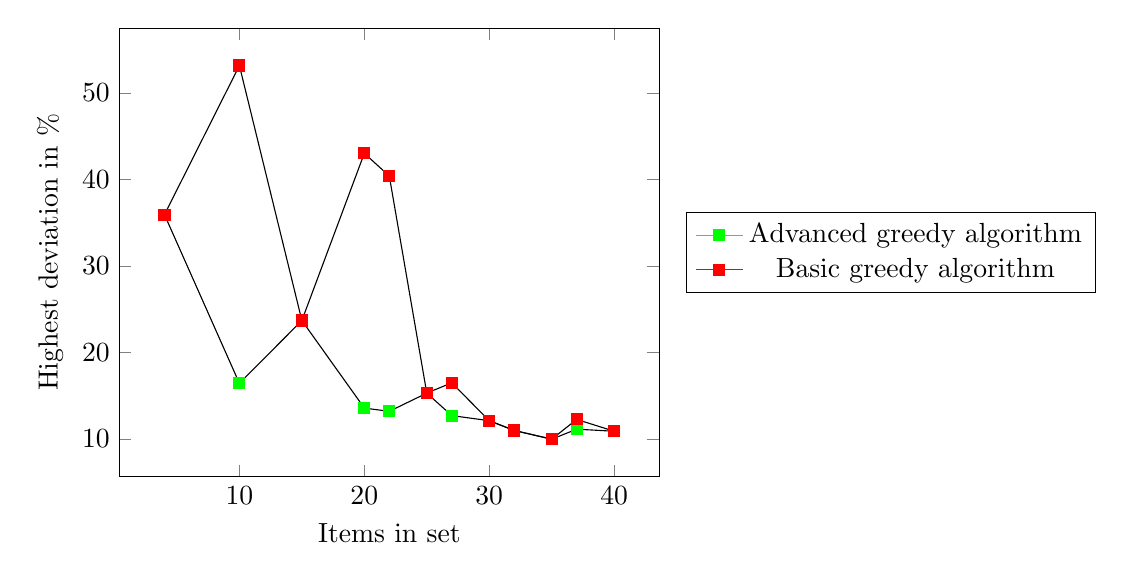
\begin{tikzpicture}
		\begin{axis}[
			xlabel=Items in set,
			ylabel=Highest deviation in \%,
			scatter/classes={
				% fptas1={mark=square*,blue},
				advancedGreedy1={mark=square*,green},
				solveHungry1={mark=square*,red}
				}
            ]
% \addplot[scatter,scatter src=explicit symbolic]table[meta=label] {
% x y label
% 4 0.0835 fptas1
% 10 0.009412 fptas1
% 15 0.005128 fptas1
% 20 0.0019934 fptas1
% 22 0.002894 fptas1
% 25 0.002714 fptas1
% };
\addplot[scatter,scatter src=explicit symbolic]table[meta=label] {
x y label
4 35.92 advancedGreedy1
10 16.42 advancedGreedy1
15 23.68 advancedGreedy1
20 13.56 advancedGreedy1
22 13.18 advancedGreedy1
25 15.29 advancedGreedy1
27 12.69 advancedGreedy1
30 12.1 advancedGreedy1
32 10.97 advancedGreedy1
35 9.964 advancedGreedy1
37 11.12 advancedGreedy1
40 10.88 advancedGreedy1
};
\addplot[scatter,scatter src=explicit symbolic]table[meta=label] {
x y label
4 35.92 solveHungry1
10 53.15 solveHungry1
15 23.68 solveHungry1
20 43.01 solveHungry1
22 40.38 solveHungry1
25 15.29 solveHungry1
27 16.48 solveHungry1
30 12.1 solveHungry1
32 10.97 solveHungry1
35 9.964 solveHungry1
37 12.25 solveHungry1
40 10.88 solveHungry1
};
			% \addlegendentry{FPTAS algorithm with $\epsilon = 0.1$}
			\addlegendentry{Advanced greedy algorithm}
			\addlegendentry{Basic greedy algorithm}
		\end{axis}
	\end{tikzpicture}
\caption{Highest deviation in greedy algorithms for each set of items on normal dataset}
\label{plot:maxDev}
\end{figure}
